\PassOptionsToPackage{unicode=true}{hyperref} % options for packages loaded elsewhere
\PassOptionsToPackage{hyphens}{url}
%
\documentclass[
]{article}
\usepackage{lmodern}
\usepackage{amssymb,amsmath}
\usepackage{ifxetex,ifluatex}
\ifnum 0\ifxetex 1\fi\ifluatex 1\fi=0 % if pdftex
  \usepackage[T1]{fontenc}
  \usepackage[utf8]{inputenc}
  \usepackage{textcomp} % provides euro and other symbols
\else % if luatex or xelatex
  \usepackage{unicode-math}
  \defaultfontfeatures{Scale=MatchLowercase}
  \defaultfontfeatures[\rmfamily]{Ligatures=TeX,Scale=1}
\fi
% use upquote if available, for straight quotes in verbatim environments
\IfFileExists{upquote.sty}{\usepackage{upquote}}{}
\IfFileExists{microtype.sty}{% use microtype if available
  \usepackage[]{microtype}
  \UseMicrotypeSet[protrusion]{basicmath} % disable protrusion for tt fonts
}{}
\makeatletter
\@ifundefined{KOMAClassName}{% if non-KOMA class
  \IfFileExists{parskip.sty}{%
    \usepackage{parskip}
  }{% else
    \setlength{\parindent}{0pt}
    \setlength{\parskip}{6pt plus 2pt minus 1pt}}
}{% if KOMA class
  \KOMAoptions{parskip=half}}
\makeatother
\usepackage{xcolor}
\IfFileExists{xurl.sty}{\usepackage{xurl}}{} % add URL line breaks if available
\IfFileExists{bookmark.sty}{\usepackage{bookmark}}{\usepackage{hyperref}}
\hypersetup{
  pdftitle={Logistic Regression Analysis},
  pdfauthor={Yalin Yang},
  pdfborder={0 0 0},
  breaklinks=true}
\urlstyle{same}  % don't use monospace font for urls
\usepackage[margin=1in]{geometry}
\usepackage{color}
\usepackage{fancyvrb}
\newcommand{\VerbBar}{|}
\newcommand{\VERB}{\Verb[commandchars=\\\{\}]}
\DefineVerbatimEnvironment{Highlighting}{Verbatim}{commandchars=\\\{\}}
% Add ',fontsize=\small' for more characters per line
\usepackage{framed}
\definecolor{shadecolor}{RGB}{248,248,248}
\newenvironment{Shaded}{\begin{snugshade}}{\end{snugshade}}
\newcommand{\AlertTok}[1]{\textcolor[rgb]{0.94,0.16,0.16}{#1}}
\newcommand{\AnnotationTok}[1]{\textcolor[rgb]{0.56,0.35,0.01}{\textbf{\textit{#1}}}}
\newcommand{\AttributeTok}[1]{\textcolor[rgb]{0.77,0.63,0.00}{#1}}
\newcommand{\BaseNTok}[1]{\textcolor[rgb]{0.00,0.00,0.81}{#1}}
\newcommand{\BuiltInTok}[1]{#1}
\newcommand{\CharTok}[1]{\textcolor[rgb]{0.31,0.60,0.02}{#1}}
\newcommand{\CommentTok}[1]{\textcolor[rgb]{0.56,0.35,0.01}{\textit{#1}}}
\newcommand{\CommentVarTok}[1]{\textcolor[rgb]{0.56,0.35,0.01}{\textbf{\textit{#1}}}}
\newcommand{\ConstantTok}[1]{\textcolor[rgb]{0.00,0.00,0.00}{#1}}
\newcommand{\ControlFlowTok}[1]{\textcolor[rgb]{0.13,0.29,0.53}{\textbf{#1}}}
\newcommand{\DataTypeTok}[1]{\textcolor[rgb]{0.13,0.29,0.53}{#1}}
\newcommand{\DecValTok}[1]{\textcolor[rgb]{0.00,0.00,0.81}{#1}}
\newcommand{\DocumentationTok}[1]{\textcolor[rgb]{0.56,0.35,0.01}{\textbf{\textit{#1}}}}
\newcommand{\ErrorTok}[1]{\textcolor[rgb]{0.64,0.00,0.00}{\textbf{#1}}}
\newcommand{\ExtensionTok}[1]{#1}
\newcommand{\FloatTok}[1]{\textcolor[rgb]{0.00,0.00,0.81}{#1}}
\newcommand{\FunctionTok}[1]{\textcolor[rgb]{0.00,0.00,0.00}{#1}}
\newcommand{\ImportTok}[1]{#1}
\newcommand{\InformationTok}[1]{\textcolor[rgb]{0.56,0.35,0.01}{\textbf{\textit{#1}}}}
\newcommand{\KeywordTok}[1]{\textcolor[rgb]{0.13,0.29,0.53}{\textbf{#1}}}
\newcommand{\NormalTok}[1]{#1}
\newcommand{\OperatorTok}[1]{\textcolor[rgb]{0.81,0.36,0.00}{\textbf{#1}}}
\newcommand{\OtherTok}[1]{\textcolor[rgb]{0.56,0.35,0.01}{#1}}
\newcommand{\PreprocessorTok}[1]{\textcolor[rgb]{0.56,0.35,0.01}{\textit{#1}}}
\newcommand{\RegionMarkerTok}[1]{#1}
\newcommand{\SpecialCharTok}[1]{\textcolor[rgb]{0.00,0.00,0.00}{#1}}
\newcommand{\SpecialStringTok}[1]{\textcolor[rgb]{0.31,0.60,0.02}{#1}}
\newcommand{\StringTok}[1]{\textcolor[rgb]{0.31,0.60,0.02}{#1}}
\newcommand{\VariableTok}[1]{\textcolor[rgb]{0.00,0.00,0.00}{#1}}
\newcommand{\VerbatimStringTok}[1]{\textcolor[rgb]{0.31,0.60,0.02}{#1}}
\newcommand{\WarningTok}[1]{\textcolor[rgb]{0.56,0.35,0.01}{\textbf{\textit{#1}}}}
\usepackage{graphicx,grffile}
\makeatletter
\def\maxwidth{\ifdim\Gin@nat@width>\linewidth\linewidth\else\Gin@nat@width\fi}
\def\maxheight{\ifdim\Gin@nat@height>\textheight\textheight\else\Gin@nat@height\fi}
\makeatother
% Scale images if necessary, so that they will not overflow the page
% margins by default, and it is still possible to overwrite the defaults
% using explicit options in \includegraphics[width, height, ...]{}
\setkeys{Gin}{width=\maxwidth,height=\maxheight,keepaspectratio}
\setlength{\emergencystretch}{3em}  % prevent overfull lines
\providecommand{\tightlist}{%
  \setlength{\itemsep}{0pt}\setlength{\parskip}{0pt}}
\setcounter{secnumdepth}{-2}
% Redefines (sub)paragraphs to behave more like sections
\ifx\paragraph\undefined\else
  \let\oldparagraph\paragraph
  \renewcommand{\paragraph}[1]{\oldparagraph{#1}\mbox{}}
\fi
\ifx\subparagraph\undefined\else
  \let\oldsubparagraph\subparagraph
  \renewcommand{\subparagraph}[1]{\oldsubparagraph{#1}\mbox{}}
\fi

% set default figure placement to htbp
\makeatletter
\def\fps@figure{htbp}
\makeatother


\title{Logistic Regression Analysis}
\author{Yalin Yang}
\date{2020-05-11}

\begin{document}
\maketitle

{
\setcounter{tocdepth}{3}
\tableofcontents
}
\hypertarget{logits-to-probability}{%
\section{Logits to Probability}\label{logits-to-probability}}

Logits \(\in [+6,-6]\) and Regression line as \$ y = \beta\_0 + \beta\_1
* Logits\$

\begin{Shaded}
\begin{Highlighting}[]
\CommentTok{## linear form in x}
\NormalTok{b0 <-}\StringTok{ }\DecValTok{1}   \CommentTok{# Play with different parameters to see their effects on the Probs}
\CommentTok{# b0 <- 0}
\NormalTok{b1 <-}\StringTok{ }\DecValTok{5}

\NormalTok{x <-}\StringTok{ }\KeywordTok{seq}\NormalTok{((}\OperatorTok{-}\DecValTok{6}\OperatorTok{-}\NormalTok{b0)}\OperatorTok{/}\NormalTok{b1,(}\DecValTok{6}\OperatorTok{-}\NormalTok{b0)}\OperatorTok{/}\NormalTok{b1,}\DataTypeTok{length.out=}\DecValTok{200}\NormalTok{)  }\CommentTok{# Adjusted scale to b0 and b1}
\CommentTok{#x <- seq((-40-b0),(40-b0),length.out=200)  # Adjusted scale to b0 and b1}
\NormalTok{L <-}\StringTok{ }\NormalTok{b0}\OperatorTok{+}\NormalTok{b1}\OperatorTok{*}\NormalTok{x}
\end{Highlighting}
\end{Shaded}

\hypertarget{different-forms-for-p-and-1-p}{%
\subsection{Different forms for p and
(1-p)}\label{different-forms-for-p-and-1-p}}

\begin{Shaded}
\begin{Highlighting}[]
\CommentTok{## Probs of first category}
\NormalTok{p1 <-}\StringTok{ }\DecValTok{1}\OperatorTok{/}\NormalTok{(}\DecValTok{1}\OperatorTok{+}\KeywordTok{exp}\NormalTok{(}\OperatorTok{-}\NormalTok{L))}
\NormalTok{p2 <-}\StringTok{ }\KeywordTok{exp}\NormalTok{(L)}\OperatorTok{/}\NormalTok{(}\DecValTok{1}\OperatorTok{+}\KeywordTok{exp}\NormalTok{(L))}

\CommentTok{## Probs of second category}
\NormalTok{np1 <-}\StringTok{ }\DecValTok{1}\OperatorTok{/}\NormalTok{(}\DecValTok{1}\OperatorTok{+}\KeywordTok{exp}\NormalTok{(L))}
\NormalTok{np2 <-}\StringTok{ }\KeywordTok{exp}\NormalTok{(}\OperatorTok{-}\NormalTok{L)}\OperatorTok{/}\NormalTok{(}\DecValTok{1}\OperatorTok{+}\KeywordTok{exp}\NormalTok{(}\OperatorTok{-}\NormalTok{L))}

\CommentTok{## Logistic curve turning point}
\NormalTok{medX <-}\StringTok{ }\OperatorTok{-}\NormalTok{b0}\OperatorTok{/}\NormalTok{b1}
\end{Highlighting}
\end{Shaded}

\hypertarget{plot-for-different-functional-forms}{%
\subsection{Plot for different functional
forms}\label{plot-for-different-functional-forms}}

\begin{Shaded}
\begin{Highlighting}[]
\KeywordTok{layout}\NormalTok{(}\KeywordTok{matrix}\NormalTok{(}\DecValTok{1}\OperatorTok{:}\DecValTok{2}\NormalTok{,}\DataTypeTok{nrow=}\DecValTok{1}\NormalTok{,}\DataTypeTok{ncol=}\DecValTok{2}\NormalTok{))}
  \CommentTok{## Prob(Success)}
  \KeywordTok{plot}\NormalTok{(x,p1,}\DataTypeTok{ylab=}\StringTok{"1/(1+exp(-L))"}\NormalTok{,}\DataTypeTok{ylim=}\KeywordTok{c}\NormalTok{(}\DecValTok{0}\NormalTok{,}\DecValTok{1}\NormalTok{),}\DataTypeTok{type=}\StringTok{"l"}\NormalTok{, }\DataTypeTok{lwd=}\DecValTok{2}\NormalTok{, }\DataTypeTok{col=}\StringTok{"red"}\NormalTok{,}\DataTypeTok{main=}\StringTok{"Pr(X < x)"}\NormalTok{)}
  \KeywordTok{abline}\NormalTok{(}\DataTypeTok{h=}\KeywordTok{c}\NormalTok{(}\DecValTok{0}\NormalTok{,}\FloatTok{0.5}\NormalTok{,}\DecValTok{1}\NormalTok{),}\DataTypeTok{lty=}\DecValTok{2}\NormalTok{); }\KeywordTok{abline}\NormalTok{(}\DataTypeTok{v=}\NormalTok{medX,}\DataTypeTok{lty=}\DecValTok{5}\NormalTok{)}
  \CommentTok{## Prob(Failure)}
  \KeywordTok{plot}\NormalTok{(x,np1,}\DataTypeTok{ylab=}\StringTok{"1/(1+exp(L))"}\NormalTok{,}\DataTypeTok{ylim=}\KeywordTok{c}\NormalTok{(}\DecValTok{0}\NormalTok{,}\DecValTok{1}\NormalTok{),}\DataTypeTok{type=}\StringTok{"l"}\NormalTok{, }\DataTypeTok{lwd=}\DecValTok{2}\NormalTok{,}\DataTypeTok{col=}\StringTok{"blue"}\NormalTok{, }\DataTypeTok{main=}\StringTok{"1 - Pr(X < x)"}\NormalTok{)}
  \KeywordTok{abline}\NormalTok{(}\DataTypeTok{h=}\KeywordTok{c}\NormalTok{(}\DecValTok{0}\NormalTok{,}\FloatTok{0.5}\NormalTok{,}\DecValTok{1}\NormalTok{),}\DataTypeTok{lty=}\DecValTok{2}\NormalTok{); }\KeywordTok{abline}\NormalTok{(}\DataTypeTok{v=}\NormalTok{medX,}\DataTypeTok{lty=}\DecValTok{5}\NormalTok{)}
\end{Highlighting}
\end{Shaded}

\includegraphics{Lecture07_files/figure-latex/unnamed-chunk-3-1.pdf}

\begin{Shaded}
\begin{Highlighting}[]
\KeywordTok{layout}\NormalTok{(}\KeywordTok{matrix}\NormalTok{(}\DecValTok{1}\NormalTok{,}\DataTypeTok{nrow=}\DecValTok{1}\NormalTok{,}\DataTypeTok{ncol=}\DecValTok{1}\NormalTok{))}
\end{Highlighting}
\end{Shaded}

\hypertarget{check-equality-of-logit-against-l}{%
\subsection{Check equality of logit against
L}\label{check-equality-of-logit-against-l}}

\begin{Shaded}
\begin{Highlighting}[]
\KeywordTok{all.equal}\NormalTok{(L,}\KeywordTok{log}\NormalTok{(p1}\OperatorTok{/}\NormalTok{np1))}
\end{Highlighting}
\end{Shaded}

\begin{verbatim}
## [1] TRUE
\end{verbatim}

\hypertarget{logistic-regression-analysis-binary-output}{%
\section{Logistic Regression Analysis {[}Binary
output{]}}\label{logistic-regression-analysis-binary-output}}

\hypertarget{quick-look-of-dataset}{%
\subsection{Quick Look of dataset}\label{quick-look-of-dataset}}

\begin{Shaded}
\begin{Highlighting}[]
\KeywordTok{library}\NormalTok{(car)}
\end{Highlighting}
\end{Shaded}

\begin{verbatim}
## Loading required package: carData
\end{verbatim}

\begin{Shaded}
\begin{Highlighting}[]
\NormalTok{CloseVote <-}\StringTok{ }\NormalTok{foreign}\OperatorTok{::}\KeywordTok{read.spss}\NormalTok{(}\StringTok{"G:}\CharTok{\textbackslash{}\textbackslash{}}\StringTok{UTD_Classes}\CharTok{\textbackslash{}\textbackslash{}}\StringTok{2020Spring}\CharTok{\textbackslash{}\textbackslash{}}\StringTok{GISC7310_AdvancedDataAnalysis}\CharTok{\textbackslash{}\textbackslash{}}\StringTok{07Logistic Regression Analysis}\CharTok{\textbackslash{}\textbackslash{}}\StringTok{SchoolClosing.sav"}\NormalTok{, }\DataTypeTok{to.data.frame=}\OtherTok{TRUE}\NormalTok{)}

\CommentTok{## Evaluate which variables are factors}
\KeywordTok{sapply}\NormalTok{(CloseVote,is.factor)}
\end{Highlighting}
\end{Shaded}

\begin{verbatim}
##  close  lived   educ contam    hsc female   kids  nodad 
##   TRUE  FALSE  FALSE   TRUE   TRUE   TRUE   TRUE   TRUE
\end{verbatim}

Exploratory plots: barwidth \emph{proportional} to the NumOfObs in
interval

\begin{Shaded}
\begin{Highlighting}[]
\KeywordTok{par}\NormalTok{(}\DataTypeTok{mfrow =} \KeywordTok{c}\NormalTok{(}\DecValTok{2}\NormalTok{,}\DecValTok{2}\NormalTok{))}
\KeywordTok{plot}\NormalTok{(close}\OperatorTok{~}\NormalTok{lived, }\DataTypeTok{data=}\NormalTok{CloseVote)}
\KeywordTok{plot}\NormalTok{(close}\OperatorTok{~}\NormalTok{educ, }\DataTypeTok{data=}\NormalTok{CloseVote)}
\KeywordTok{plot}\NormalTok{(close}\OperatorTok{~}\NormalTok{contam, }\DataTypeTok{data=}\NormalTok{CloseVote)}
\KeywordTok{plot}\NormalTok{(close}\OperatorTok{~}\NormalTok{hsc, }\DataTypeTok{data=}\NormalTok{CloseVote)}
\end{Highlighting}
\end{Shaded}

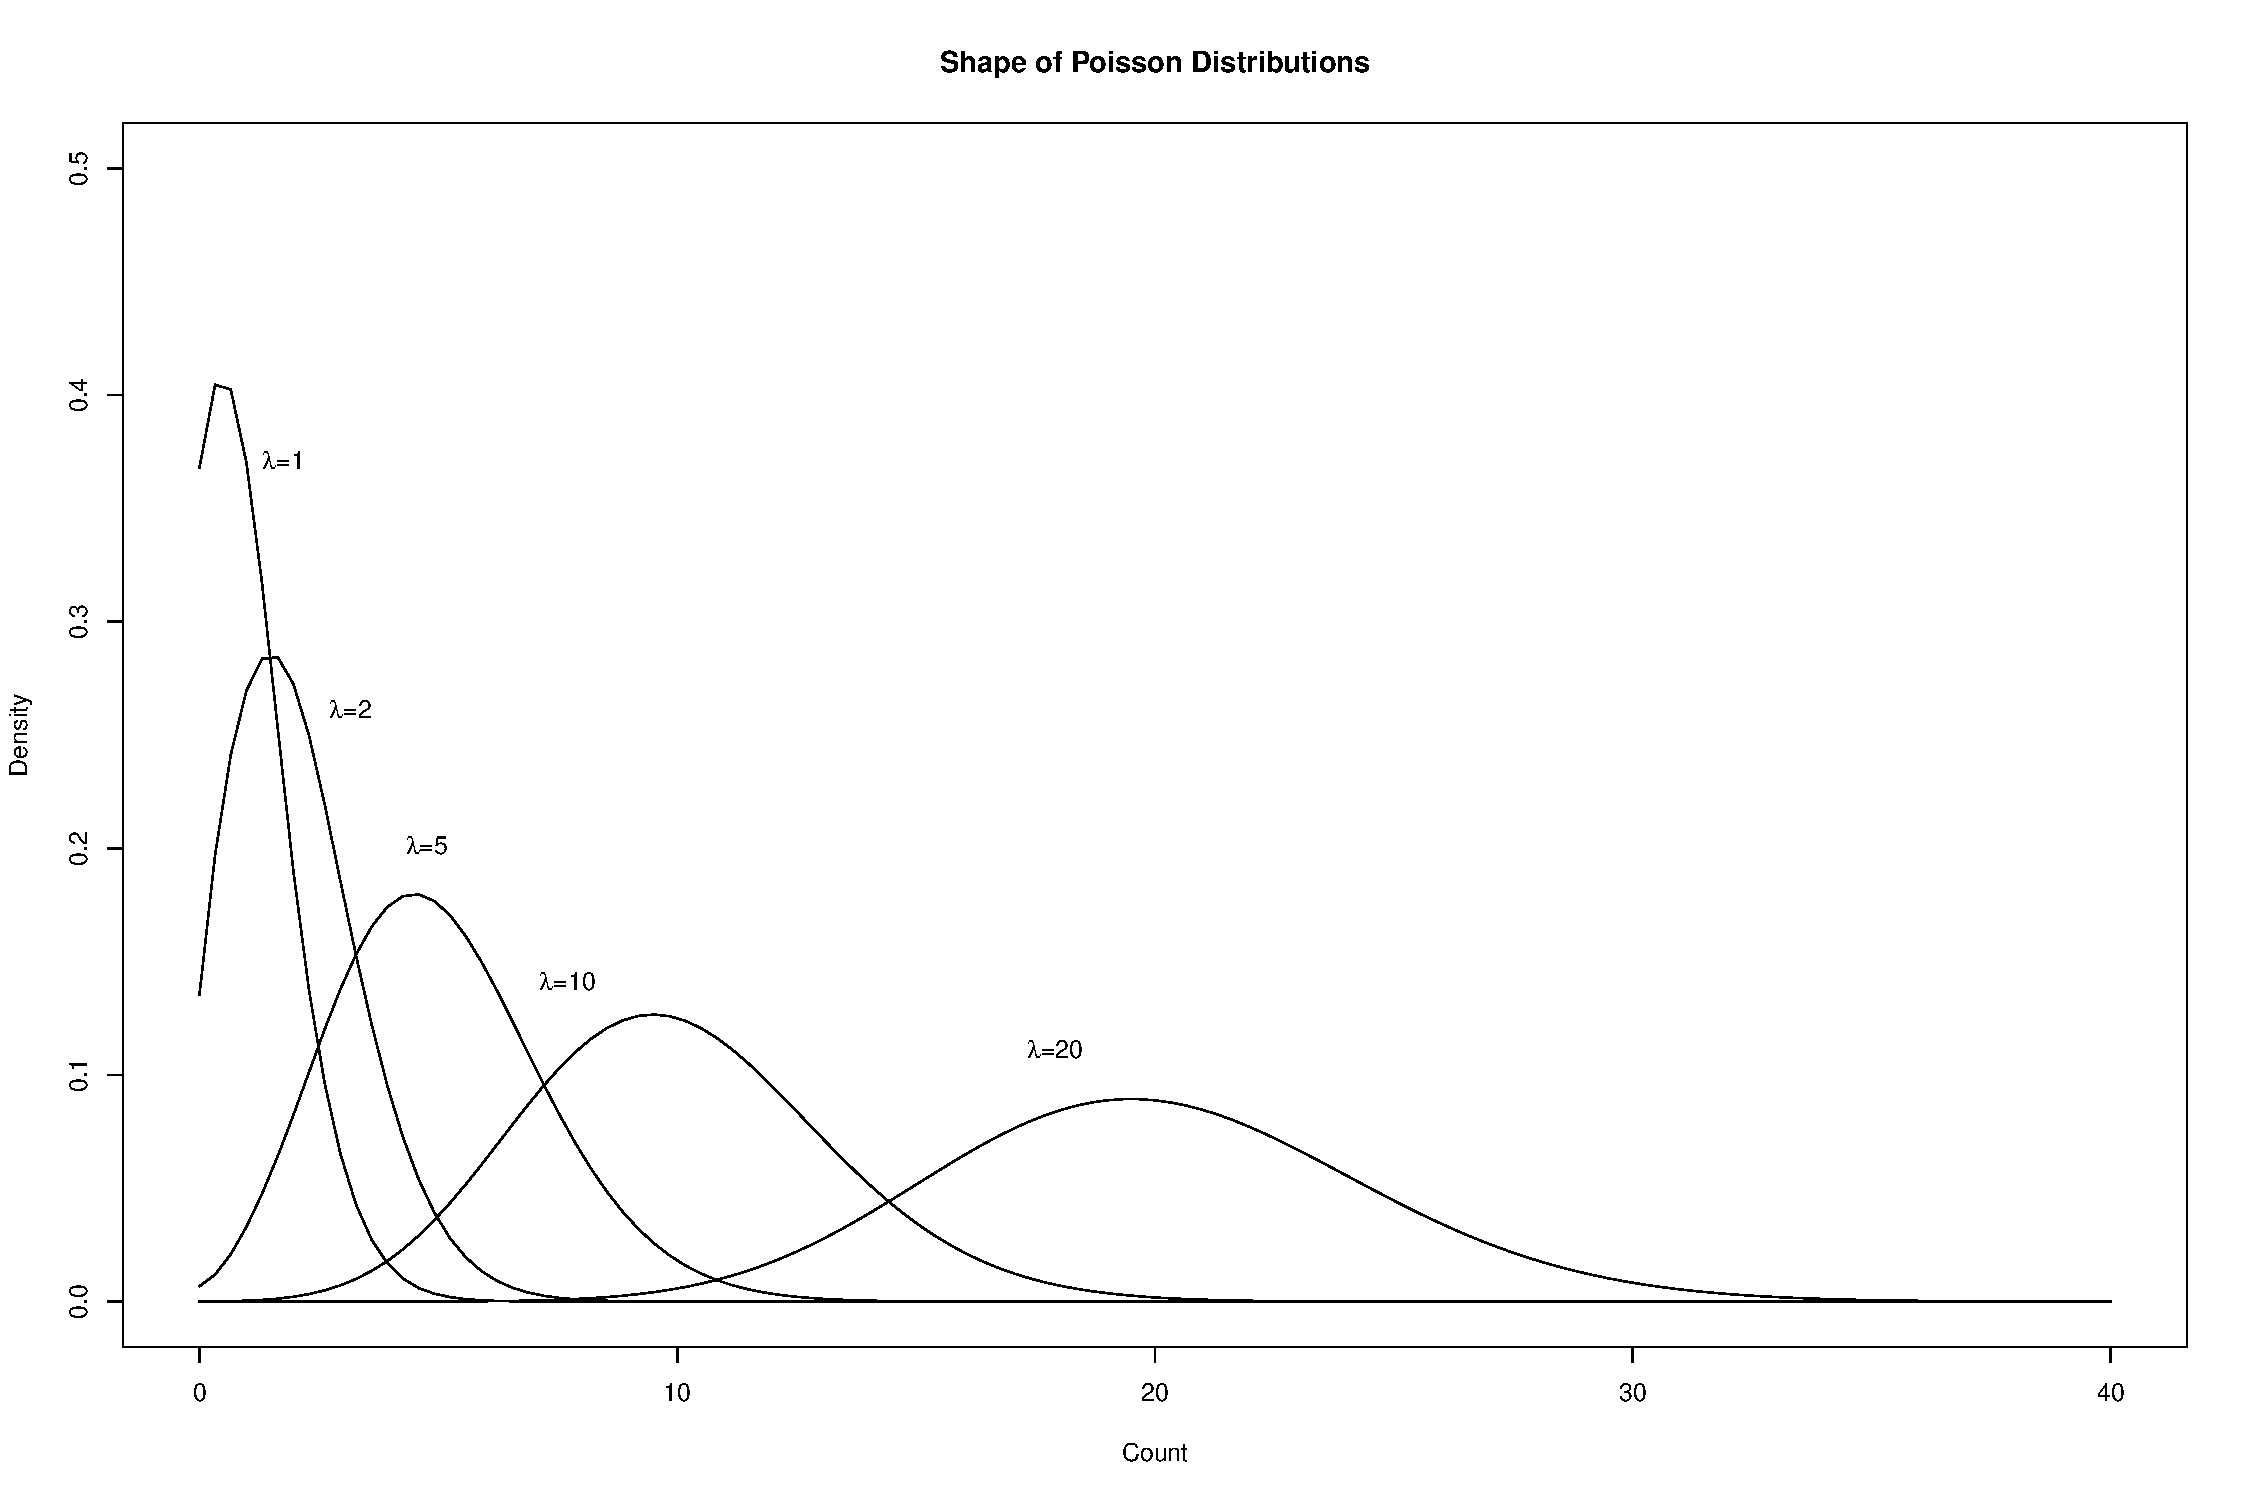
\includegraphics{Lecture07_files/figure-latex/unnamed-chunk-6-1.pdf}

\begin{Shaded}
\begin{Highlighting}[]
\KeywordTok{plot}\NormalTok{(close}\OperatorTok{~}\NormalTok{female, }\DataTypeTok{data=}\NormalTok{CloseVote)}
\KeywordTok{plot}\NormalTok{(close}\OperatorTok{~}\NormalTok{kids, }\DataTypeTok{data=}\NormalTok{CloseVote)}
\KeywordTok{plot}\NormalTok{(close}\OperatorTok{~}\NormalTok{nodad, }\DataTypeTok{data=}\NormalTok{CloseVote)}
\end{Highlighting}
\end{Shaded}

\includegraphics{Lecture07_files/figure-latex/unnamed-chunk-6-2.pdf}

\hypertarget{logistic-modeling}{%
\subsection{Logistic modeling}\label{logistic-modeling}}

Just intercept an intercept model

\begin{Shaded}
\begin{Highlighting}[]
\CommentTok{## generalize linear model}
\NormalTok{GLM}\FloatTok{.00}\NormalTok{ <-}\StringTok{ }\KeywordTok{glm}\NormalTok{(close }\OperatorTok{~}\StringTok{ }\DecValTok{1}\NormalTok{, }\DataTypeTok{family=}\KeywordTok{binomial}\NormalTok{(logit), }\DataTypeTok{trace=}\OtherTok{TRUE}\NormalTok{, }\DataTypeTok{data=}\NormalTok{CloseVote) }\CommentTok{# just intersecpt}
\end{Highlighting}
\end{Shaded}

\begin{verbatim}
## Deviance = 209.3355 Iterations - 1
## Deviance = 209.2116 Iterations - 2
## Deviance = 209.2116 Iterations - 3
## Deviance = 209.2116 Iterations - 4
\end{verbatim}

\begin{Shaded}
\begin{Highlighting}[]
\KeywordTok{summary}\NormalTok{(GLM}\FloatTok{.00}\NormalTok{)}
\end{Highlighting}
\end{Shaded}

\begin{verbatim}
## 
## Call:
## glm(formula = close ~ 1, family = binomial(logit), data = CloseVote, 
##     trace = TRUE)
## 
## Deviance Residuals: 
##    Min      1Q  Median      3Q     Max  
## -1.063  -1.063  -1.063   1.297   1.297  
## 
## Coefficients:
##             Estimate Std. Error z value Pr(>|z|)  
## (Intercept)  -0.2763     0.1632  -1.692   0.0906 .
## ---
## Signif. codes:  0 '***' 0.001 '**' 0.01 '*' 0.05 '.' 0.1 ' ' 1
## 
## (Dispersion parameter for binomial family taken to be 1)
## 
##     Null deviance: 209.21  on 152  degrees of freedom
## Residual deviance: 209.21  on 152  degrees of freedom
## AIC: 211.21
## 
## Number of Fisher Scoring iterations: 4
\end{verbatim}

\begin{Shaded}
\begin{Highlighting}[]
\KeywordTok{cat}\NormalTok{(}\StringTok{"Deviance: "}\NormalTok{, }\KeywordTok{logLik}\NormalTok{(GLM}\FloatTok{.00}\NormalTok{)}\OperatorTok{*-}\DecValTok{2}\NormalTok{)}
\end{Highlighting}
\end{Shaded}

\begin{verbatim}
## Deviance:  209.2116
\end{verbatim}

Tansfer intercept from logis to probability model

\begin{Shaded}
\begin{Highlighting}[]
\DecValTok{1}\OperatorTok{/}\NormalTok{(}\DecValTok{1}\OperatorTok{+}\KeywordTok{exp}\NormalTok{(}\OperatorTok{-}\NormalTok{(}\KeywordTok{coef}\NormalTok{(GLM}\FloatTok{.00}\NormalTok{)[}\DecValTok{1}\NormalTok{])))            }\CommentTok{# predicted prob in favor of closing 1/(1+exp(-b_0)) }
\end{Highlighting}
\end{Shaded}

\begin{verbatim}
## (Intercept) 
##   0.4313725
\end{verbatim}

\begin{Shaded}
\begin{Highlighting}[]
\KeywordTok{mean}\NormalTok{(}\KeywordTok{unclass}\NormalTok{(CloseVote}\OperatorTok{$}\NormalTok{close)}\OperatorTok{-}\DecValTok{1}\NormalTok{)         }\CommentTok{# same as average zeros and ones}
\end{Highlighting}
\end{Shaded}

\begin{verbatim}
## [1] 0.4313725
\end{verbatim}

Bi-variate model ``lived'' and intercept

\begin{Shaded}
\begin{Highlighting}[]
\NormalTok{GLM}\FloatTok{.01}\NormalTok{ <-}\StringTok{ }\KeywordTok{glm}\NormalTok{(close }\OperatorTok{~}\StringTok{ }\NormalTok{lived, }\DataTypeTok{family=}\KeywordTok{binomial}\NormalTok{(logit), }\DataTypeTok{trace=}\OtherTok{TRUE}\NormalTok{, }\DataTypeTok{data=}\NormalTok{CloseVote)}
\end{Highlighting}
\end{Shaded}

\begin{verbatim}
## Deviance = 195.2677 Iterations - 1
## Deviance = 195.2671 Iterations - 2
## Deviance = 195.2671 Iterations - 3
\end{verbatim}

\begin{Shaded}
\begin{Highlighting}[]
\KeywordTok{summary}\NormalTok{(GLM}\FloatTok{.01}\NormalTok{)  }\CommentTok{#slope is for logit, not for probability}
\end{Highlighting}
\end{Shaded}

\begin{verbatim}
## 
## Call:
## glm(formula = close ~ lived, family = binomial(logit), data = CloseVote, 
##     trace = TRUE)
## 
## Deviance Residuals: 
##     Min       1Q   Median       3Q      Max  
## -1.3597  -1.0619  -0.6094   1.1049   2.2001  
## 
## Coefficients:
##             Estimate Std. Error z value Pr(>|z|)    
## (Intercept)  0.45998    0.26257   1.752 0.079797 .  
## lived       -0.04099    0.01214  -3.376 0.000735 ***
## ---
## Signif. codes:  0 '***' 0.001 '**' 0.01 '*' 0.05 '.' 0.1 ' ' 1
## 
## (Dispersion parameter for binomial family taken to be 1)
## 
##     Null deviance: 209.21  on 152  degrees of freedom
## Residual deviance: 195.27  on 151  degrees of freedom
## AIC: 199.27
## 
## Number of Fisher Scoring iterations: 3
\end{verbatim}

\begin{Shaded}
\begin{Highlighting}[]
\KeywordTok{cat}\NormalTok{(}\StringTok{"Deviance: "}\NormalTok{, }\DecValTok{-2}\OperatorTok{*}\KeywordTok{logLik}\NormalTok{(GLM}\FloatTok{.01}\NormalTok{))}
\end{Highlighting}
\end{Shaded}

\begin{verbatim}
## Deviance:  195.2671
\end{verbatim}

\hypertarget{likelihood-ratio-test}{%
\subsection{Likelihood Ratio Test}\label{likelihood-ratio-test}}

The ``hard'' way

\begin{Shaded}
\begin{Highlighting}[]
\NormalTok{( LR <-}\StringTok{ }\DecValTok{-2}\OperatorTok{*}\NormalTok{(}\KeywordTok{logLik}\NormalTok{(GLM}\FloatTok{.00}\NormalTok{)}\OperatorTok{-}\KeywordTok{logLik}\NormalTok{(GLM}\FloatTok{.01}\NormalTok{)) )}
\end{Highlighting}
\end{Shaded}

\begin{verbatim}
## 'log Lik.' 13.94442 (df=1)
\end{verbatim}

\begin{Shaded}
\begin{Highlighting}[]
\NormalTok{( }\KeywordTok{pchisq}\NormalTok{(LR[}\DecValTok{1}\NormalTok{], }\DataTypeTok{df=}\DecValTok{1}\NormalTok{, }\DataTypeTok{lower.tail=}\NormalTok{F) )}
\end{Highlighting}
\end{Shaded}

\begin{verbatim}
## [1] 0.0001882954
\end{verbatim}

The ``easy'' way

\begin{Shaded}
\begin{Highlighting}[]
\KeywordTok{anova}\NormalTok{(GLM}\FloatTok{.00}\NormalTok{,GLM}\FloatTok{.01}\NormalTok{,}\DataTypeTok{test=}\StringTok{"LRT"}\NormalTok{)}
\end{Highlighting}
\end{Shaded}

\begin{verbatim}
## Analysis of Deviance Table
## 
## Model 1: close ~ 1
## Model 2: close ~ lived
##   Resid. Df Resid. Dev Df Deviance  Pr(>Chi)    
## 1       152     209.21                          
## 2       151     195.27  1   13.944 0.0001883 ***
## ---
## Signif. codes:  0 '***' 0.001 '**' 0.01 '*' 0.05 '.' 0.1 ' ' 1
\end{verbatim}

\hypertarget{alternative-the-probit-model}{%
\subsection{Alternative: The probit
model}\label{alternative-the-probit-model}}

\begin{Shaded}
\begin{Highlighting}[]
\NormalTok{GLM.probit <-}\StringTok{ }\KeywordTok{glm}\NormalTok{(close }\OperatorTok{~}\StringTok{ }\NormalTok{lived, }\DataTypeTok{family=}\KeywordTok{binomial}\NormalTok{(}\DataTypeTok{link=}\NormalTok{probit), }\DataTypeTok{trace=}\OtherTok{TRUE}\NormalTok{, }\DataTypeTok{data=}\NormalTok{CloseVote)}
\end{Highlighting}
\end{Shaded}

\begin{verbatim}
## Deviance = 195.376 Iterations - 1
## Deviance = 195.375 Iterations - 2
## Deviance = 195.375 Iterations - 3
\end{verbatim}

\begin{Shaded}
\begin{Highlighting}[]
\KeywordTok{summary}\NormalTok{(GLM.probit)}
\end{Highlighting}
\end{Shaded}

\begin{verbatim}
## 
## Call:
## glm(formula = close ~ lived, family = binomial(link = probit), 
##     data = CloseVote, trace = TRUE)
## 
## Deviance Residuals: 
##    Min      1Q  Median      3Q     Max  
## -1.351  -1.066  -0.612   1.109   2.237  
## 
## Coefficients:
##              Estimate Std. Error z value Pr(>|z|)    
## (Intercept)  0.273851   0.160573   1.705 0.088109 .  
## lived       -0.024499   0.007014  -3.493 0.000477 ***
## ---
## Signif. codes:  0 '***' 0.001 '**' 0.01 '*' 0.05 '.' 0.1 ' ' 1
## 
## (Dispersion parameter for binomial family taken to be 1)
## 
##     Null deviance: 209.21  on 152  degrees of freedom
## Residual deviance: 195.38  on 151  degrees of freedom
## AIC: 199.38
## 
## Number of Fisher Scoring iterations: 3
\end{verbatim}

\begin{Shaded}
\begin{Highlighting}[]
\KeywordTok{logLik}\NormalTok{(GLM.probit)}
\end{Highlighting}
\end{Shaded}

\begin{verbatim}
## 'log Lik.' -97.68752 (df=2)
\end{verbatim}

\hypertarget{full-model-and-restricted-model}{%
\subsection{Full model and Restricted
model}\label{full-model-and-restricted-model}}

Full model with all variables and interaction term nodad

\begin{Shaded}
\begin{Highlighting}[]
\NormalTok{GLM}\FloatTok{.02}\NormalTok{ <-}\StringTok{ }\KeywordTok{glm}\NormalTok{(close }\OperatorTok{~}\StringTok{ }\NormalTok{lived }\OperatorTok{+}\StringTok{ }\NormalTok{educ }\OperatorTok{+}\StringTok{ }\NormalTok{contam }\OperatorTok{+}\StringTok{ }\NormalTok{hsc }\OperatorTok{+}\StringTok{ }\NormalTok{nodad }\OperatorTok{+}\StringTok{ }\NormalTok{female }\OperatorTok{+}\StringTok{ }\NormalTok{kids ,}
              \DataTypeTok{family=}\KeywordTok{binomial}\NormalTok{(logit), }\DataTypeTok{trace=}\OtherTok{TRUE}\NormalTok{, }\DataTypeTok{data=}\NormalTok{CloseVote)}
\end{Highlighting}
\end{Shaded}

\begin{verbatim}
## Deviance = 143.5404 Iterations - 1
## Deviance = 141.1452 Iterations - 2
## Deviance = 141.0496 Iterations - 3
## Deviance = 141.0494 Iterations - 4
## Deviance = 141.0494 Iterations - 5
\end{verbatim}

\begin{Shaded}
\begin{Highlighting}[]
\KeywordTok{summary}\NormalTok{(GLM}\FloatTok{.02}\NormalTok{, }\DataTypeTok{correlation=}\NormalTok{F)}
\end{Highlighting}
\end{Shaded}

\begin{verbatim}
## 
## Call:
## glm(formula = close ~ lived + educ + contam + hsc + nodad + female + 
##     kids, family = binomial(logit), data = CloseVote, trace = TRUE)
## 
## Deviance Residuals: 
##     Min       1Q   Median       3Q      Max  
## -2.6027  -0.7557  -0.3091   0.6316   2.3920  
## 
## Coefficients:
##              Estimate Std. Error z value Pr(>|z|)    
## (Intercept)   2.89372    1.60298   1.805  0.07104 .  
## lived        -0.04664    0.01698  -2.748  0.00600 ** 
## educ         -0.20602    0.09320  -2.211  0.02706 *  
## contamyes     1.28208    0.48137   2.663  0.00774 ** 
## hscyes        2.41800    0.50966   4.744 2.09e-06 ***
## nodadyes     -2.22599    0.99911  -2.228  0.02588 *  
## femalefemale -0.05156    0.55712  -0.093  0.92626    
## kidsyes      -0.67062    0.56561  -1.186  0.23576    
## ---
## Signif. codes:  0 '***' 0.001 '**' 0.01 '*' 0.05 '.' 0.1 ' ' 1
## 
## (Dispersion parameter for binomial family taken to be 1)
## 
##     Null deviance: 209.21  on 152  degrees of freedom
## Residual deviance: 141.05  on 145  degrees of freedom
## AIC: 157.05
## 
## Number of Fisher Scoring iterations: 5
\end{verbatim}

\begin{Shaded}
\begin{Highlighting}[]
\KeywordTok{vif}\NormalTok{(GLM}\FloatTok{.02}\NormalTok{)}
\end{Highlighting}
\end{Shaded}

\begin{verbatim}
##    lived     educ   contam      hsc    nodad   female     kids 
## 1.332797 1.205248 1.044889 1.127165 2.036254 1.573675 1.746393
\end{verbatim}

\begin{Shaded}
\begin{Highlighting}[]
\KeywordTok{logLik}\NormalTok{(GLM}\FloatTok{.02}\NormalTok{)}
\end{Highlighting}
\end{Shaded}

\begin{verbatim}
## 'log Lik.' -70.52469 (df=8)
\end{verbatim}

\begin{Shaded}
\begin{Highlighting}[]
\CommentTok{# confint(GLM.02, level=0.95, type="Wald")}
\end{Highlighting}
\end{Shaded}

Restricted model without female and kids

\begin{Shaded}
\begin{Highlighting}[]
\NormalTok{GLM}\FloatTok{.03}\NormalTok{ <-}\StringTok{ }\KeywordTok{glm}\NormalTok{(close }\OperatorTok{~}\StringTok{ }\NormalTok{lived }\OperatorTok{+}\StringTok{ }\NormalTok{educ }\OperatorTok{+}\StringTok{ }\NormalTok{contam }\OperatorTok{+}\StringTok{ }\NormalTok{hsc }\OperatorTok{+}\StringTok{ }\NormalTok{nodad ,}
             \DataTypeTok{family=}\KeywordTok{binomial}\NormalTok{(logit), }\DataTypeTok{data=}\NormalTok{CloseVote,}
             \DataTypeTok{control=}\KeywordTok{list}\NormalTok{(}\DataTypeTok{epsilon=}\FloatTok{1e-15}\NormalTok{,}\DataTypeTok{maxit=}\DecValTok{50}\NormalTok{, }\DataTypeTok{trace=}\OtherTok{TRUE}\NormalTok{))}
\end{Highlighting}
\end{Shaded}

\begin{verbatim}
## Deviance = 144.7235 Iterations - 1
## Deviance = 142.7147 Iterations - 2
## Deviance = 142.6526 Iterations - 3
## Deviance = 142.6525 Iterations - 4
## Deviance = 142.6525 Iterations - 5
## Deviance = 142.6525 Iterations - 6
\end{verbatim}

\begin{Shaded}
\begin{Highlighting}[]
\KeywordTok{summary}\NormalTok{(GLM}\FloatTok{.03}\NormalTok{, }\DataTypeTok{correlation=}\OtherTok{TRUE}\NormalTok{)}
\end{Highlighting}
\end{Shaded}

\begin{verbatim}
## 
## Call:
## glm(formula = close ~ lived + educ + contam + hsc + nodad, family = binomial(logit), 
##     data = CloseVote, control = list(epsilon = 1e-15, maxit = 50, 
##         trace = TRUE))
## 
## Deviance Residuals: 
##     Min       1Q   Median       3Q      Max  
## -2.6053  -0.7485  -0.3211   0.6320   2.4202  
## 
## Coefficients:
##             Estimate Std. Error z value Pr(>|z|)    
## (Intercept)  2.18227    1.33014   1.641  0.10087    
## lived       -0.03965    0.01548  -2.561  0.01043 *  
## educ        -0.19667    0.09261  -2.124  0.03371 *  
## contamyes    1.29855    0.47663   2.724  0.00644 ** 
## hscyes       2.27855    0.49037   4.647 3.37e-06 ***
## nodadyes    -1.73095    0.72527  -2.387  0.01700 *  
## ---
## Signif. codes:  0 '***' 0.001 '**' 0.01 '*' 0.05 '.' 0.1 ' ' 1
## 
## (Dispersion parameter for binomial family taken to be 1)
## 
##     Null deviance: 209.21  on 152  degrees of freedom
## Residual deviance: 142.65  on 147  degrees of freedom
## AIC: 154.65
## 
## Number of Fisher Scoring iterations: 6
## 
## Correlation of Coefficients:
##           (Intercept) lived educ  contamyes hscyes
## lived     -0.48                                   
## educ      -0.96        0.33                       
## contamyes -0.02       -0.07 -0.06                 
## hscyes     0.07       -0.03 -0.16 -0.02           
## nodadyes  -0.16       -0.08  0.17 -0.17     -0.17
\end{verbatim}

\begin{Shaded}
\begin{Highlighting}[]
\KeywordTok{logLik}\NormalTok{(GLM}\FloatTok{.03}\NormalTok{)}
\end{Highlighting}
\end{Shaded}

\begin{verbatim}
## 'log Lik.' -71.32623 (df=6)
\end{verbatim}

\hypertarget{likelihood-ratio-test-1}{%
\subsubsection{Likelihood Ratio Test}\label{likelihood-ratio-test-1}}

\begin{Shaded}
\begin{Highlighting}[]
\KeywordTok{anova}\NormalTok{(GLM}\FloatTok{.03}\NormalTok{,GLM}\FloatTok{.02}\NormalTok{,}\DataTypeTok{test=}\StringTok{"LRT"}\NormalTok{)}
\end{Highlighting}
\end{Shaded}

\begin{verbatim}
## Analysis of Deviance Table
## 
## Model 1: close ~ lived + educ + contam + hsc + nodad
## Model 2: close ~ lived + educ + contam + hsc + nodad + female + kids
##   Resid. Df Resid. Dev Df Deviance Pr(>Chi)
## 1       147     142.65                     
## 2       145     141.05  2   1.6031   0.4486
\end{verbatim}

\hypertarget{effect-plots}{%
\subsection{Effect plots}\label{effect-plots}}

\begin{Shaded}
\begin{Highlighting}[]
\KeywordTok{library}\NormalTok{(effects)}
\end{Highlighting}
\end{Shaded}

\begin{verbatim}
## Registered S3 methods overwritten by 'lme4':
##   method                          from
##   cooks.distance.influence.merMod car 
##   influence.merMod                car 
##   dfbeta.influence.merMod         car 
##   dfbetas.influence.merMod        car
\end{verbatim}

\begin{verbatim}
## lattice theme set by effectsTheme()
## See ?effectsTheme for details.
\end{verbatim}

\begin{Shaded}
\begin{Highlighting}[]
\CommentTok{## all independent variables with the others at average. }
\CommentTok{## Note type="response" for probability scale}
\KeywordTok{plot}\NormalTok{(}\KeywordTok{allEffects}\NormalTok{(GLM}\FloatTok{.03}\NormalTok{), }\DataTypeTok{type=}\StringTok{"response"}\NormalTok{, }\DataTypeTok{ylim=}\KeywordTok{c}\NormalTok{(}\DecValTok{0}\NormalTok{,}\DecValTok{1}\NormalTok{), }\DataTypeTok{ask=}\OtherTok{FALSE}\NormalTok{)}
\end{Highlighting}
\end{Shaded}

\includegraphics{Lecture07_files/figure-latex/unnamed-chunk-16-1.pdf}

\begin{Shaded}
\begin{Highlighting}[]
\CommentTok{## Group specifice effect plots}
\KeywordTok{summary}\NormalTok{(CloseVote)}
\end{Highlighting}
\end{Shaded}

\begin{verbatim}
##    close        lived            educ       contam     hsc         female  
##  open :87   Min.   : 1.00   Min.   : 6.00   no :110   no :106   male  :60  
##  close:66   1st Qu.: 5.00   1st Qu.:12.00   yes: 43   yes: 47   female:93  
##             Median :15.00   Median :12.00                                  
##             Mean   :19.27   Mean   :12.95                                  
##             3rd Qu.:29.00   3rd Qu.:15.00                                  
##             Max.   :81.00   Max.   :20.00                                  
##   kids    nodad    
##  no :63   no :127  
##  yes:90   yes: 26  
##                    
##                    
##                    
## 
\end{verbatim}

\hypertarget{low-prob-respondent}{%
\subsubsection{Low prob respondent}\label{low-prob-respondent}}

\begin{Shaded}
\begin{Highlighting}[]
\NormalTok{eff.GLM.low <-}\StringTok{ }\KeywordTok{effect}\NormalTok{(}\StringTok{"lived"}\NormalTok{,GLM}\FloatTok{.03}\NormalTok{,}
                      \DataTypeTok{given.values=}\KeywordTok{c}\NormalTok{(}\DataTypeTok{educ=}\DecValTok{20}\NormalTok{,}\StringTok{"contamyes"}\NormalTok{=}\DecValTok{0}\NormalTok{,}\StringTok{"hscyes"}\NormalTok{=}\DecValTok{0}\NormalTok{,}\StringTok{"nodadyes"}\NormalTok{=}\DecValTok{1}\NormalTok{))}
\KeywordTok{plot}\NormalTok{(eff.GLM.low, }\DataTypeTok{type=}\StringTok{"response"}\NormalTok{, }\DataTypeTok{ylim=}\KeywordTok{c}\NormalTok{(}\DecValTok{0}\NormalTok{,}\DecValTok{1}\NormalTok{), }\DataTypeTok{ylab=}\KeywordTok{expression}\NormalTok{(}\KeywordTok{Pr}\NormalTok{(Y[i]}\OperatorTok{==}\StringTok{"Close"}\NormalTok{)), }
     \DataTypeTok{main=}\StringTok{"Low Probability Respondents"}\NormalTok{)}
\end{Highlighting}
\end{Shaded}

\includegraphics{Lecture07_files/figure-latex/unnamed-chunk-18-1.pdf}

\hypertarget{average-prob-respondent}{%
\subsubsection{Average prob respondent}\label{average-prob-respondent}}

\begin{Shaded}
\begin{Highlighting}[]
\NormalTok{eff.GLM.average <-}\StringTok{ }\KeywordTok{effect}\NormalTok{(}\StringTok{"lived"}\NormalTok{,GLM}\FloatTok{.03}\NormalTok{)}
\KeywordTok{plot}\NormalTok{(eff.GLM.average, }\DataTypeTok{ylim=}\KeywordTok{c}\NormalTok{(}\DecValTok{0}\NormalTok{,}\DecValTok{1}\NormalTok{), }\DataTypeTok{type=}\StringTok{"response"}\NormalTok{, }\DataTypeTok{ylab=}\KeywordTok{expression}\NormalTok{(}\KeywordTok{Pr}\NormalTok{(Y[i]}\OperatorTok{==}\StringTok{"Close"}\NormalTok{)),    }\CommentTok{# ylim is in terms of probs}
     \DataTypeTok{main=}\StringTok{"Average Probability Respondents"}\NormalTok{)}
\end{Highlighting}
\end{Shaded}

\includegraphics{Lecture07_files/figure-latex/unnamed-chunk-19-1.pdf}

\hypertarget{high-prob-respondent}{%
\subsubsection{High prob respondent}\label{high-prob-respondent}}

\begin{Shaded}
\begin{Highlighting}[]
\NormalTok{eff.GLM.hi <-}\StringTok{ }\KeywordTok{effect}\NormalTok{(}\StringTok{"lived"}\NormalTok{,GLM}\FloatTok{.03}\NormalTok{,}
                     \DataTypeTok{given.values=}\KeywordTok{c}\NormalTok{(}\DataTypeTok{educ=}\DecValTok{6}\NormalTok{,}\StringTok{"contamyes"}\NormalTok{=}\DecValTok{1}\NormalTok{,}\StringTok{"hscyes"}\NormalTok{=}\DecValTok{1}\NormalTok{,}\StringTok{"nodadyes"}\NormalTok{=}\DecValTok{0}\NormalTok{))}
\KeywordTok{plot}\NormalTok{(eff.GLM.hi, }\DataTypeTok{type=}\StringTok{"response"}\NormalTok{, }\DataTypeTok{ylim=}\KeywordTok{c}\NormalTok{(}\DecValTok{0}\NormalTok{,}\DecValTok{1}\NormalTok{), }\DataTypeTok{ylab=}\KeywordTok{expression}\NormalTok{(}\KeywordTok{Pr}\NormalTok{(Y[i]}\OperatorTok{==}\StringTok{"Close"}\NormalTok{)), }
     \DataTypeTok{main=}\StringTok{"High Probability Respondents"}\NormalTok{)}
\end{Highlighting}
\end{Shaded}

\includegraphics{Lecture07_files/figure-latex/unnamed-chunk-20-1.pdf}

\hypertarget{residual-exploration}{%
\section{Residual Exploration}\label{residual-exploration}}

\hypertarget{response-residuals}{%
\subsection{Response Residuals}\label{response-residuals}}

\begin{Shaded}
\begin{Highlighting}[]
\NormalTok{resid.GLM}\FloatTok{.03}\NormalTok{ <-}\StringTok{ }\KeywordTok{residuals}\NormalTok{(GLM}\FloatTok{.03}\NormalTok{, }\DataTypeTok{type=}\StringTok{"response"}\NormalTok{)   }\CommentTok{# check ?residuals.glm}
\NormalTok{pred.GLM}\FloatTok{.03}\NormalTok{ <-}\StringTok{ }\KeywordTok{predict}\NormalTok{(GLM}\FloatTok{.03}\NormalTok{, }\DataTypeTok{type=}\StringTok{"response"}\NormalTok{)      }\CommentTok{# check ?predict.glm}
\KeywordTok{plot}\NormalTok{(pred.GLM}\FloatTok{.03}\NormalTok{, resid.GLM}\FloatTok{.03}\NormalTok{, }\DataTypeTok{ylim=}\KeywordTok{c}\NormalTok{(}\OperatorTok{-}\DecValTok{1}\NormalTok{,}\DecValTok{1}\NormalTok{), }\DataTypeTok{xlim=}\KeywordTok{c}\NormalTok{(}\DecValTok{0}\NormalTok{,}\DecValTok{1}\NormalTok{), }
     \DataTypeTok{ylab=}\StringTok{"Response Residuals"}\NormalTok{, }\DataTypeTok{xlab=}\StringTok{"Predicted Probabilities"}\NormalTok{)}
\KeywordTok{abline}\NormalTok{(}\DataTypeTok{h=}\DecValTok{0}\NormalTok{, }\DataTypeTok{lty=}\DecValTok{5}\NormalTok{)}
\KeywordTok{lines}\NormalTok{(}\KeywordTok{lowess}\NormalTok{(pred.GLM}\FloatTok{.03}\NormalTok{, resid.GLM}\FloatTok{.03}\NormalTok{),}\DataTypeTok{lwd=}\DecValTok{2}\NormalTok{)  }\CommentTok{# Smoothed function to see the residual behavior}
\end{Highlighting}
\end{Shaded}

\includegraphics{Lecture07_files/figure-latex/unnamed-chunk-21-1.pdf}

\hypertarget{pearson-residuals-standardized-residuals}{%
\subsection{Pearson Residuals (standardized
residuals)}\label{pearson-residuals-standardized-residuals}}

\begin{Shaded}
\begin{Highlighting}[]
\NormalTok{resid.GLM}\FloatTok{.03}\NormalTok{ <-}\StringTok{ }\KeywordTok{residuals}\NormalTok{(GLM}\FloatTok{.03}\NormalTok{, }\DataTypeTok{type=}\StringTok{"pearson"}\NormalTok{)   }
\NormalTok{pred.GLM}\FloatTok{.03}\NormalTok{ <-}\StringTok{ }\KeywordTok{predict}\NormalTok{(GLM}\FloatTok{.03}\NormalTok{, }\DataTypeTok{type=}\StringTok{"response"}\NormalTok{)      }
\KeywordTok{plot}\NormalTok{(pred.GLM}\FloatTok{.03}\NormalTok{, resid.GLM}\FloatTok{.03}\NormalTok{, }\DataTypeTok{xlim=}\KeywordTok{c}\NormalTok{(}\DecValTok{0}\NormalTok{,}\DecValTok{1}\NormalTok{), }
     \DataTypeTok{ylab=}\StringTok{"Pearson Residuals"}\NormalTok{, }\DataTypeTok{xlab=}\StringTok{"Predicted Probabilities"}\NormalTok{)}
\KeywordTok{abline}\NormalTok{(}\DataTypeTok{h=}\DecValTok{0}\NormalTok{, }\DataTypeTok{lty=}\DecValTok{5}\NormalTok{)}
\KeywordTok{lines}\NormalTok{(}\KeywordTok{lowess}\NormalTok{(pred.GLM}\FloatTok{.03}\NormalTok{, resid.GLM}\FloatTok{.03}\NormalTok{),}\DataTypeTok{lwd=}\DecValTok{2}\NormalTok{)  }\CommentTok{# Smoothed function to see the residual behavior}
\end{Highlighting}
\end{Shaded}

\includegraphics{Lecture07_files/figure-latex/unnamed-chunk-22-1.pdf}

\hypertarget{logistic-regression-analysis-rates}{%
\section{Logistic Regression Analysis
{[}Rates{]}}\label{logistic-regression-analysis-rates}}

Weighted GLM specification

\begin{Shaded}
\begin{Highlighting}[]
\NormalTok{insects <-}\StringTok{ }\KeywordTok{data.frame}\NormalTok{(}\DataTypeTok{popDensity=}\KeywordTok{c}\NormalTok{(}\DecValTok{1}\NormalTok{,}\DecValTok{4}\NormalTok{,}\DecValTok{10}\NormalTok{,}\DecValTok{22}\NormalTok{,}\DecValTok{55}\NormalTok{,}\DecValTok{121}\NormalTok{,}\DecValTok{210}\NormalTok{,}\DecValTok{444}\NormalTok{),}
                      \DataTypeTok{females=}\KeywordTok{c}\NormalTok{(}\DecValTok{1}\NormalTok{,}\DecValTok{3}\NormalTok{,}\DecValTok{7}\NormalTok{,}\DecValTok{18}\NormalTok{,}\DecValTok{22}\NormalTok{,}\DecValTok{41}\NormalTok{,}\DecValTok{52}\NormalTok{,}\DecValTok{79}\NormalTok{),}
                      \DataTypeTok{males=}\KeywordTok{c}\NormalTok{(}\DecValTok{0}\NormalTok{,}\DecValTok{1}\NormalTok{,}\DecValTok{3}\NormalTok{,}\DecValTok{4}\NormalTok{,}\DecValTok{33}\NormalTok{,}\DecValTok{80}\NormalTok{,}\DecValTok{158}\NormalTok{,}\DecValTok{365}\NormalTok{))}

\NormalTok{insects}\OperatorTok{$}\NormalTok{totalPop <-}\StringTok{ }\NormalTok{insects}\OperatorTok{$}\NormalTok{females}\OperatorTok{+}\NormalTok{insects}\OperatorTok{$}\NormalTok{males}
\NormalTok{insects}\OperatorTok{$}\NormalTok{rateMale <-}\StringTok{ }\NormalTok{insects}\OperatorTok{$}\NormalTok{males}\OperatorTok{/}\NormalTok{insects}\OperatorTok{$}\NormalTok{totalPop}
\NormalTok{glm.weight <-}\StringTok{ }\KeywordTok{glm}\NormalTok{(rateMale}\OperatorTok{~}\KeywordTok{log}\NormalTok{(popDensity), }\DataTypeTok{weights=}\NormalTok{totalPop, }\DataTypeTok{data=}\NormalTok{insects, }\DataTypeTok{family=}\NormalTok{binomial)}
\KeywordTok{summary}\NormalTok{(glm.weight)}
\end{Highlighting}
\end{Shaded}

\begin{verbatim}
## 
## Call:
## glm(formula = rateMale ~ log(popDensity), family = binomial, 
##     data = insects, weights = totalPop)
## 
## Deviance Residuals: 
##     Min       1Q   Median       3Q      Max  
## -1.9697  -0.3411   0.1499   0.4019   1.0372  
## 
## Coefficients:
##                 Estimate Std. Error z value Pr(>|z|)    
## (Intercept)     -2.65927    0.48758  -5.454 4.92e-08 ***
## log(popDensity)  0.69410    0.09056   7.665 1.80e-14 ***
## ---
## Signif. codes:  0 '***' 0.001 '**' 0.01 '*' 0.05 '.' 0.1 ' ' 1
## 
## (Dispersion parameter for binomial family taken to be 1)
## 
##     Null deviance: 71.1593  on 7  degrees of freedom
## Residual deviance:  5.6739  on 6  degrees of freedom
## AIC: 38.201
## 
## Number of Fisher Scoring iterations: 4
\end{verbatim}

\begin{Shaded}
\begin{Highlighting}[]
\CommentTok{## Plot prediction}
\NormalTok{xAxis <-}\StringTok{ }\KeywordTok{seq}\NormalTok{(}\DecValTok{0}\NormalTok{,}\DecValTok{7}\NormalTok{,}\DataTypeTok{by=}\FloatTok{0.001}\NormalTok{)                                                    }\CommentTok{# value range of log(popDensity)}
\NormalTok{probPred <-}\StringTok{ }\KeywordTok{predict}\NormalTok{(glm.weight,}\KeywordTok{list}\NormalTok{(}\DataTypeTok{popDensity=}\KeywordTok{exp}\NormalTok{(xAxis)), }\DataTypeTok{type=}\StringTok{"response"}\NormalTok{)   }\CommentTok{# type="response" give predicted probabilities}
\KeywordTok{plot}\NormalTok{(}\KeywordTok{log}\NormalTok{(insects}\OperatorTok{$}\NormalTok{popDensity), insects}\OperatorTok{$}\NormalTok{rateMale, }\DataTypeTok{ylim=}\KeywordTok{c}\NormalTok{(}\DecValTok{0}\NormalTok{,}\DecValTok{1}\NormalTok{), }\DataTypeTok{xlim=}\KeywordTok{c}\NormalTok{(}\DecValTok{0}\NormalTok{,}\DecValTok{7}\NormalTok{), }
     \DataTypeTok{ylab=}\KeywordTok{expression}\NormalTok{(}\KeywordTok{Pr}\NormalTok{(Y[i] }\OperatorTok{==}\StringTok{"Male"}\NormalTok{)),}\DataTypeTok{xlab=}\KeywordTok{expression}\NormalTok{(}\KeywordTok{log}\NormalTok{(}\StringTok{"Population Density"}\NormalTok{)), }
     \DataTypeTok{pch=}\DecValTok{16}\NormalTok{, }\DataTypeTok{col=}\StringTok{"blue"}\NormalTok{)}
\KeywordTok{lines}\NormalTok{(xAxis,probPred, }\DataTypeTok{col=}\StringTok{"red"}\NormalTok{)}
\KeywordTok{abline}\NormalTok{(}\DataTypeTok{h=}\KeywordTok{c}\NormalTok{(}\DecValTok{0}\NormalTok{,}\DecValTok{1}\NormalTok{),}\DataTypeTok{lty=}\DecValTok{3}\NormalTok{)}
\end{Highlighting}
\end{Shaded}

\includegraphics{Lecture07_files/figure-latex/unnamed-chunk-24-1.pdf}

\end{document}
